\documentclass{article}
\usepackage[T1]{fontenc}
\usepackage{lmodern}
\usepackage{graphicx}
\usepackage{amsmath,amssymb}
\usepackage[a4paper,margin=2cm]{geometry}
\usepackage[absolute,overlay]{textpos}
\setlength{\TPHorizModule}{1mm}
\setlength{\TPVertModule}{1mm}
\usepackage[indonesian]{babel}
\usepackage{hyperref}
\setlength{\emergencystretch}{2em}
% unit: Halaman 85

\begin{document}

% === Halaman 85 (llm) ===

\section*{1 RIFF Header (12 byte pertama)}

\vspace{80.19mm}

Bagian ini adalah identitas file.

\vspace{5mm}

Artinya:
\begin{itemize}
    \item \texttt{''RIFF''} $\rightarrow$ format container
    \item \texttt{''WAVE''} $\rightarrow$ tipe file audio
\end{itemize}

\begin{flushright}
Sumber: ChatGPT
\end{flushright}

% deskripsi: Tabel struktur RIFF Header yang menunjukkan offset, ukuran, dan isi untuk byte 0-11.
% bbox normalisasi: [0.1250, 0.2900, 0.7050, 0.5600]
\begin{textblock*}{121.80mm}(26.25mm,86.13mm)
\noindent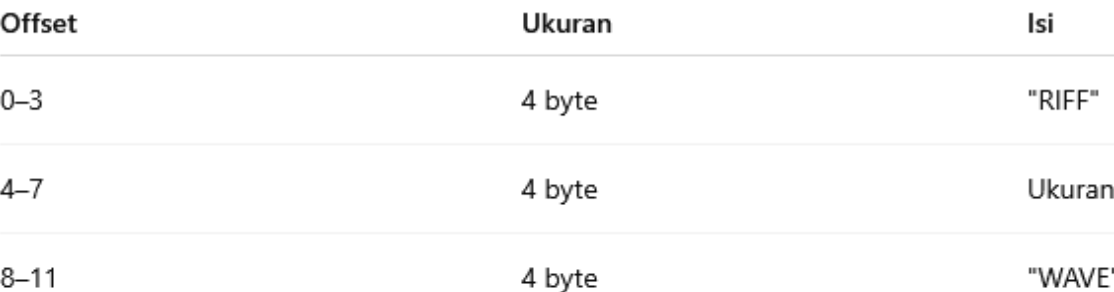
\includegraphics[width=121.80mm,height=80.19mm]{../../images/llm/page_085_img_01.png}%
\end{textblock*}

\end{document}
